\chapter{Materiais e Métodos}
    \label{cap-materiais}    
    
    O método \MT proposto por \citeauthor{tikhonov50} \citeyearpar{tikhonov50} e
    \citeauthor{cagniard53} \citeyearpar{cagniard53}, usa as propriedades
    eletromagnéticas para estudar a distribuição de resistividade na crosta, 
    podendo variar a sua investigação de dezenas de metros a dezenas de 
    quilômetros.
    
    \section{Origem das Correntes Telúricas}
    
    As flutuações no campo magnético terrestre geram campos elétricos na alta atmosfera que induzem correntes magnéticas, as ondas eletromagnéticas então penetram no interior da Terra na forma de ondas planas ortogonais que induzem novas correntes chamadas de corrente telúricas que trazem informações das características físicas das litologias. 
    
    Uma das características é a modulação da frenquência, causada por diferentes tipos de rochas e estruturas, esse fenômeno é diretamente 
	relacionado a resistividade do meio. \textcolor{red}{citar}
    
    As frequências das ondas são baixas variando de 1 $mHz$ à 10 $kHz$, ondas com frequências menores que 1 $Hz$ tem origem nos ventos solares que interagem como o campo magnético terrestre, já ondas com frequências maiores de 1 $Hz$ são provocadas por tempestades equatoriais.\textcolor{red}{citar  relação, e regras meio isotrpico}
    
%RESISTIVIDADE ==============================================================================================================================================
    \section{Resistividade dos Materiais}
    
    Para o \MT a propriedade de contraste investigada é a condutividade[$\sigma$] ou resistividade[$\rho$] sendo essa o inverso da condutividade.
    A resistividade é uma propriedade particular de cada material, ou seja, a partir de uma resistividade podemos estimar a qual material ela pertence\footnote{Para os meios geológicos essa propriedade é representada por um intervalo de valores, devido as complexidades químicas e físicas das diferentes litologias.}.
    
    Em 1827, Georg Ohm verificou de forma empírica que aplicando uma diferença de potencial em um material esse gera uma resistência a passagem de corrente, essa relação é chamada de lei de Ohm (equação \ref{lei_de_ohm})\textcolor{red}{citar}.
    
    \begin{equation}
     \label{lei_de_ohm}
     V = R i
    \end{equation}
    
    Onde $V$ é a diferença de potencial [V], $i$ é a corrente [A] e $R$ é a resistência [$\Omega$], materiais que obedecem essa lei são chamados de materiais ômicos, a Terra é considerada um material ômico, porem para a investigação geofísica a resistência não é uma propriedade viável, visto  que depende muito da geometria do problema, assim foi proposto a resistividade, onde, um mesmo material terá a sua resistividade igual independente da geometria.
    
    A resistividade então é definida pela \textcolor{red}{ que o material oferece para um comprimento (equação \ref{resistividade})........ mudar isso e colocar igual do livro}, a figura \ref{fig_resistividade} mostra um circuito para se obter a resistividade, sendo A a área ($m^2$), R a resistência ($\Omega$), L o comprimento ($m$) e $\rho$ a resistividade dada em $\Omega m$. 
    
    \begin{equation}
        \label{resistividade}
        \rho = \dfrac{R A}{L}\, \, \, ;\, \, \, \, \, \, \, \, \, \, \, \, \, \,  R = \dfrac{V}{i}
    \end{equation}
    
    
    \begin{figure}[h]
        \centering
        \caption{Arranjo para medir a resistividade ($\rho$) de um material}
        \centerline{\includegraphics[width=4cm]{texto/fig/resisti_telford.png}}
        \fonte{Adaptado \citeauthor{telford}, \citeyearpar{telford}}
        \label{fig_resistividade}
    \end{figure}
    
    A figura \ref{tabela_resistividade} mostra a distribuição de resistividade para diversos materiais geológicos. 
    Portanto podemos identificar a partir de um contexto geológico quais litologias pertence a cada resistividade encontrada, por exemplo, uma litologia que tenha reistividade em torno de  $100 \, \Omega m$ e outra com $3000 \, \Omega m $ pode ser caracterízada como um arenito e uma rocha ignea respectivamente. 
    
    \begin{figure}[h]
        \centering
        \caption{Resistividade dos Materiais Geológicos}
        \centerline{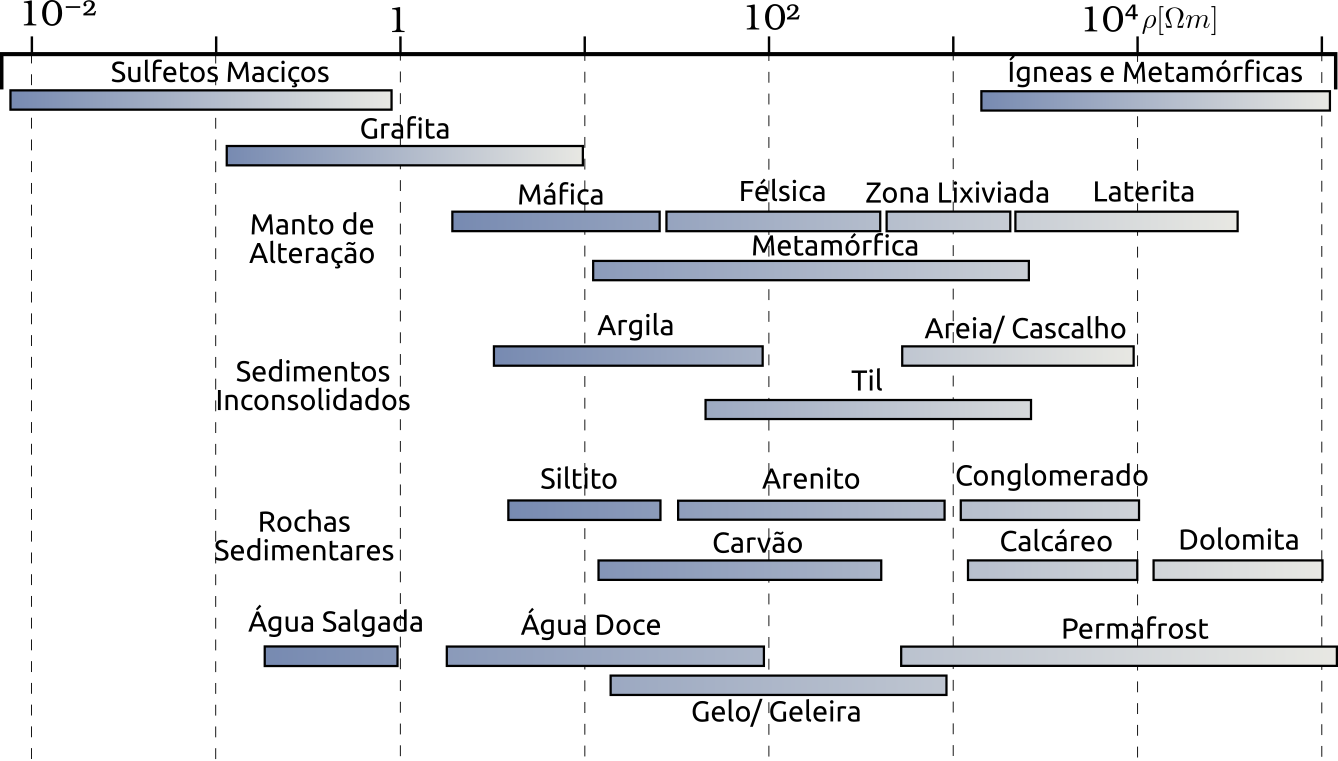
\includegraphics[width=14cm]{texto/fig/resistividade_tabela.png}}
        \fonte{Adaptado \citeauthor{eletromag_met}, \citeyearpar{eletromag_met}}
        \label{tabela_resistividade}
    \end{figure}
% FIM RESISTIVIDADE
%===========================================================================================================================================================    
    
    
    
% Eletromagneticos
%===================================================================================================================================================
    \section{Fundamentos Teóricos dos Métodos Eletromagnéticos}
        Apoiado nas leis de Maxwell \cite{eletromag8hayt} podemos medir os campos elétricos e magnéticos separadamente em diferentes componentes e assim unir para obter a função de \textit{skin-depth}.
	
        Os campos podem ser descritos pelas equações a seguir\footnote{Para cargas e correntes livres
        (macroscópica)}:
            \begin{equation}
                \label{rot_elet_max}
                \nabla \times \vec{\textrm{E}}=-\frac{\partial \vec{\textrm{B}}}{\partial t} 
            \end{equation}
            \begin{equation}
                \label{rot_mag_max}
                \nabla \times \vec{\textrm{H}} = \vec{\textrm{J}} + \frac{\partial \vec{\textrm{D}}}{\partial t}
            \end{equation}
            \begin{equation}
                \nabla \cdot \vec{\textrm{B}} = 0
            \end{equation}
            \begin{equation}
                \nabla \cdot \vec{\textrm{D}} = \rho
            \end{equation}

            $\vec{\textrm{E}}$ $\rightarrow$ Campo Elétrico [$V/m$]
	    
            $\vec{\textrm{B}}$ $\rightarrow$ Campo Magnético [$T$]
	    
            $\vec{\textrm{H}}$ $\rightarrow$ Campo Magnetizante [$A/m$]
	    
            $\vec{\textrm{J}}$ $\rightarrow$ Densidade de Corrente [$A/m^2$]
	    
            $\vec{\textrm{D}}$ $\rightarrow$ Campo de Deslocamento Elétrico [$C/m^2$]
	    
            $\rho$ $\rightarrow$ Densidade de Carga [$C/m^3$]
	    
            $t$ $\rightarrow$ Tempo [$s$]

            Obedecendo as relações de contorno para um meio isotrópico temos as seguintes
            relações (equações constitutivas):
            \begin{equation}
                \label{con_B}
                \vec{\textrm{B}} = \mu \vec{\textrm{H}}
            \end{equation}
            \begin{equation}
                \label{con_D}
                \vec{\textrm{D}} = \varepsilon  \vec{\textrm{E}}
            \end{equation}
            \begin{equation}
                \label{con_J}
                \vec{\textrm{J}} = \sigma \vec{\textrm{E}}
            \end{equation}
	    
            $\mu$ $\rightarrow$ Permeabilidade Magnética [$H/m$]
	    
            $\varepsilon$ $\rightarrow$ Permissividade Elétrica [$F/m$]
	    
            $\sigma$ $\rightarrow$ Condutividade Elétrica [$S/m$]
	    
            Cada escalar das equações anteriores são características que dependem do meio em que a onda se propaga.
	    
            Para a crosta $\mu = 1,2566\textrm{x}10^{-6} H/m$ e $\varepsilon = 8,85
            \textrm{x}10^{-12} F/m$ esses parâmetros funcionam como tensores em um meio
            anisotrópico que variam em função do tempo, já considerando para os 
            trabalhos de investigação o meio supõe-se ser isotrópico, assim, 
            tornando estáticos os tensores.
	
    
    
    
    
    
% MT
%===================================================================================================================
    \section{Resposta do Método Magnetotelúrico}
        \subsection{Impedância Eletromagnética}
        
        
        
    
    
    
    \section{Modelo de Dimensões MT}
        \subsection{Terra 1D}
        \subsection{Terra 2D}
        
        O modelo de Terra 2D é caracterizado pelo contato vertical entre dois meios de diferentes resistividades. Se o contato é
	    paralelo ao eixo $x$ então é definido a direção do \textit{strike} no eixo $x$, a direção deve ser paralela ao plano de contato,
	    ou seja, onde a condutividade é constante.% (Figura \ref{fig_strike}).
	    
	    \begin{figure}[h]
	        \caption{Modelo de Terra 2D para a resistividade variando na direção $y$}
	        \begin{center}
	        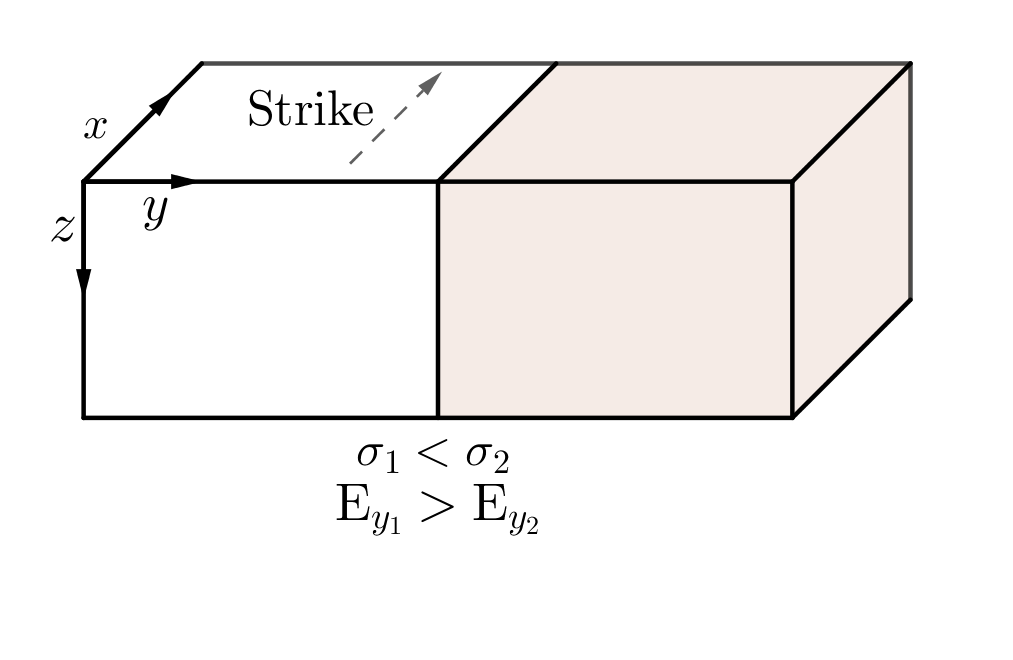
\includegraphics[width=12cm]{texto/fig/Tm_Te.png} 
	        \end{center}
		\fonte{Adaptado \cite{didana2010}}
		\label{fig_strike}
	    \end{figure}
	    Devido a essa diferença entre as resistividades polarizamos os campos em TE (Transversal Elétrico) e TM (Transversal Magnético).
	    Para esse modelo temos o tensor impedância como:
	    \begin{equation}
	     \textrm{Z}_{2D} = \left (\begin{array}{cc}
	                               0 & \textrm{Z}_{xy} \\
	                               \textrm{Z}_{yx} & 0
	                              \end{array} \right)
	    \end{equation}
	    Assim cada polarização pode ser escrita como:
	    \begin{equation}
	     \textrm{TE} = \left \{ \begin{array}{l}
	            \dfrac{\partial \textrm{E}_x}{\partial y} = \dfrac{\partial \textrm{B}_z}{\partial t} = -i\omega \textrm{B}_z \\
	           \dfrac{\partial \textrm{E}_x}{\partial z} = \dfrac{\partial \textrm{B}_y}{\partial t} = i\omega \textrm{B}_y \\
	           \dfrac{\partial \textrm{B}_z}{\partial y} - \dfrac{\partial \textrm{B}_y}{\partial z} = \mu \sigma \textrm{E}_x 
	           \end{array} \right.
	    \end{equation}
	    \begin{equation}
	     \textrm{TM} = \left \{ \begin{array}{l}
	            \dfrac{\partial \textrm{B}_x}{\partial y} = \mu \sigma \textrm{E}_z \\
	           -\dfrac{\partial \textrm{B}_x}{\partial z} = \mu \sigma \textrm{E}_y \\
	           \dfrac{\partial \textrm{E}_z}{\partial y} - \dfrac{\partial \textrm{E}_y}{\partial z} = i \omega \textrm{B}_x 
	           \end{array} \right.
	    \end{equation}
        
        
        \subsection{Terra 3D}
    
    \section{Processamento das Series Temporais (mudar o titulo)}
    
    \section{Ferramentas de Desenvolvimento do \textit{Software}}
    
        O desenvolvimento do \textit{software} foi baseado na filosofia de \textit{Software Livre} \textcolor{red}{citar} onde o código fonte será liberado e distribuído para a comunidade geofísica. A linguagem base escolhida para o projeto foi o Python, visto as vastas bibliotecas para trabalhar com dados científicos \citar{procurar o termo correto em ingles} e a simplicidade da implementação do código.  
        
        \subsection{Linguagem PYTHON}
            \label{lim_python}
            \citar{ Falar um pouco da historia do python}
            
            Exemplos de código Python:

            Mostrar conteúdo na Tela:
            
            Como comentado, o código tem fácil leitura, para imprimir um conteúdo na tela 
            podemos simplesmente usar o comando \verb|print|, aproximando muito da linguagem falada.  
            \begin{quote}
             \codbox{\ini   \cc{Comentários}                  \\
                     \ini   \f{print} ('Hello Word')          \\
                     Hello World
                     }                                          \citar{\codnum{\ref{lim_python}.1}}

            \end{quote}
            
            Operações Matemáticas:
            
            As variáveis no código não precisam ser declaradas para um 
            tipo específico (Ex.: \textit{float, int, string}), deixando assim o código mais fluido.\citar{melhorar} 
            \begin{quote}
            
             \codbox{\ini a = 2                               \\
                     \ini b = 5                               \\
                     \ini \f{print}(a + b)                    \\
                     7                                        \\
                     %\ini                                    \\
                     \ini \f{print}(b / a)                    \\
                     2.5                                      \\
                     %\ini \cl{class} Tela(App):              \\
                     %\init  \cl{return} Tela
                     }                                          \citar{\codnum{\ref{lim_python}.2}}
            \end{quote}
            
            Importando Módulos:
            
            Módulos são estruturas que podemos importar objetos de um código a outro,
            no script \citar{\ref{lim_python}.3} importamos o valor de $\pi$ que esta contido na variável \verb|pi| dentro do pacote \verb|math|. 
            
            \begin{quote}
             \codbox{\ini \cl{import} math                    \\
                     \ini                                     \\
                     \ini pi = math.pi                        \\
                     \ini \f{print}(pi)                       \\
                     3.141592653589793
                    }                                           \citar{\codnum{\ref{lim_python}.3}}
            \end{quote}
            
        \subsection{Módulos e Pacotes}
            
            A vasta quantidade de pacotes de terceiros para Python é o que faz a linguagem tão rica, os 
            pacotes facilitam a implementação do código, por exemplo, que for preciso calcular o espectro de 
            frequência de um conjunto de dados não será necessário implementar todo o algoritmo para efetuar o calculo, resolver as integrais e assim por diante, mas sim podemos utilizar o pacote \verb|scipy| e importarmos a função \verb|dnff()| que já foi implementada e executar em nosso código, esse processo economiza tempo em desenvolvimento.           
            
            \subsubsection{Kivy}
            
            
            \label{lim_kivy}
            Kivy é um \textit{framework} criado em 2010 pela KIVY ORGANIZATION \cite{kivy} e \textit{opensource} para o desenvolvimento de interfaces gráficas, a escolha dessa interface foi a alta compatibilidade entre sistemas operacionais e todo o processamento para desenhar a tela é feita no chip gráfico liberando então mais processamento pela CPU.
            
            Kivy também é uma linguagem de programação que permite a criação da interface de forma mais fácil, similar ao QT \citar{citar} ela usa uma linguagem de marcação e indentada onde as propriedades dos \textit{widgets} (Objetos interativos com o usuário) são adicionadas colocando-as a baixo e com espaçamento de 4 espaços do \textit{widget}. 
                        
            Exemplo do Kivy dentro do código Python:
            \begin{quote}
             \codbox{\ini \cl{from} kivy.app \cl{import} App                      \\
                     \ini \cl{from} kivy.uix.button \cl{import} Button            \\
                     \ini                                                         \\
                     \ini      \cl{class} Test(App):                              \\
                     \init          \cl{def} build(self):                         \\
                     \init \,\,\,\,\,\,     \cl{return} Button(\ob{text}=\st{'Hello Word')} \\
                     \ini                                                         \\
                     \ini Test().run()                                            
             }                                                                    \citar{\codnum{\ref{lim_kivy}.1}}
            \end{quote}
            
            \begin{figure}[h]
                \caption{Exemplo Janela com Kivy implementada somente com código Python}
                \begin{center}
                    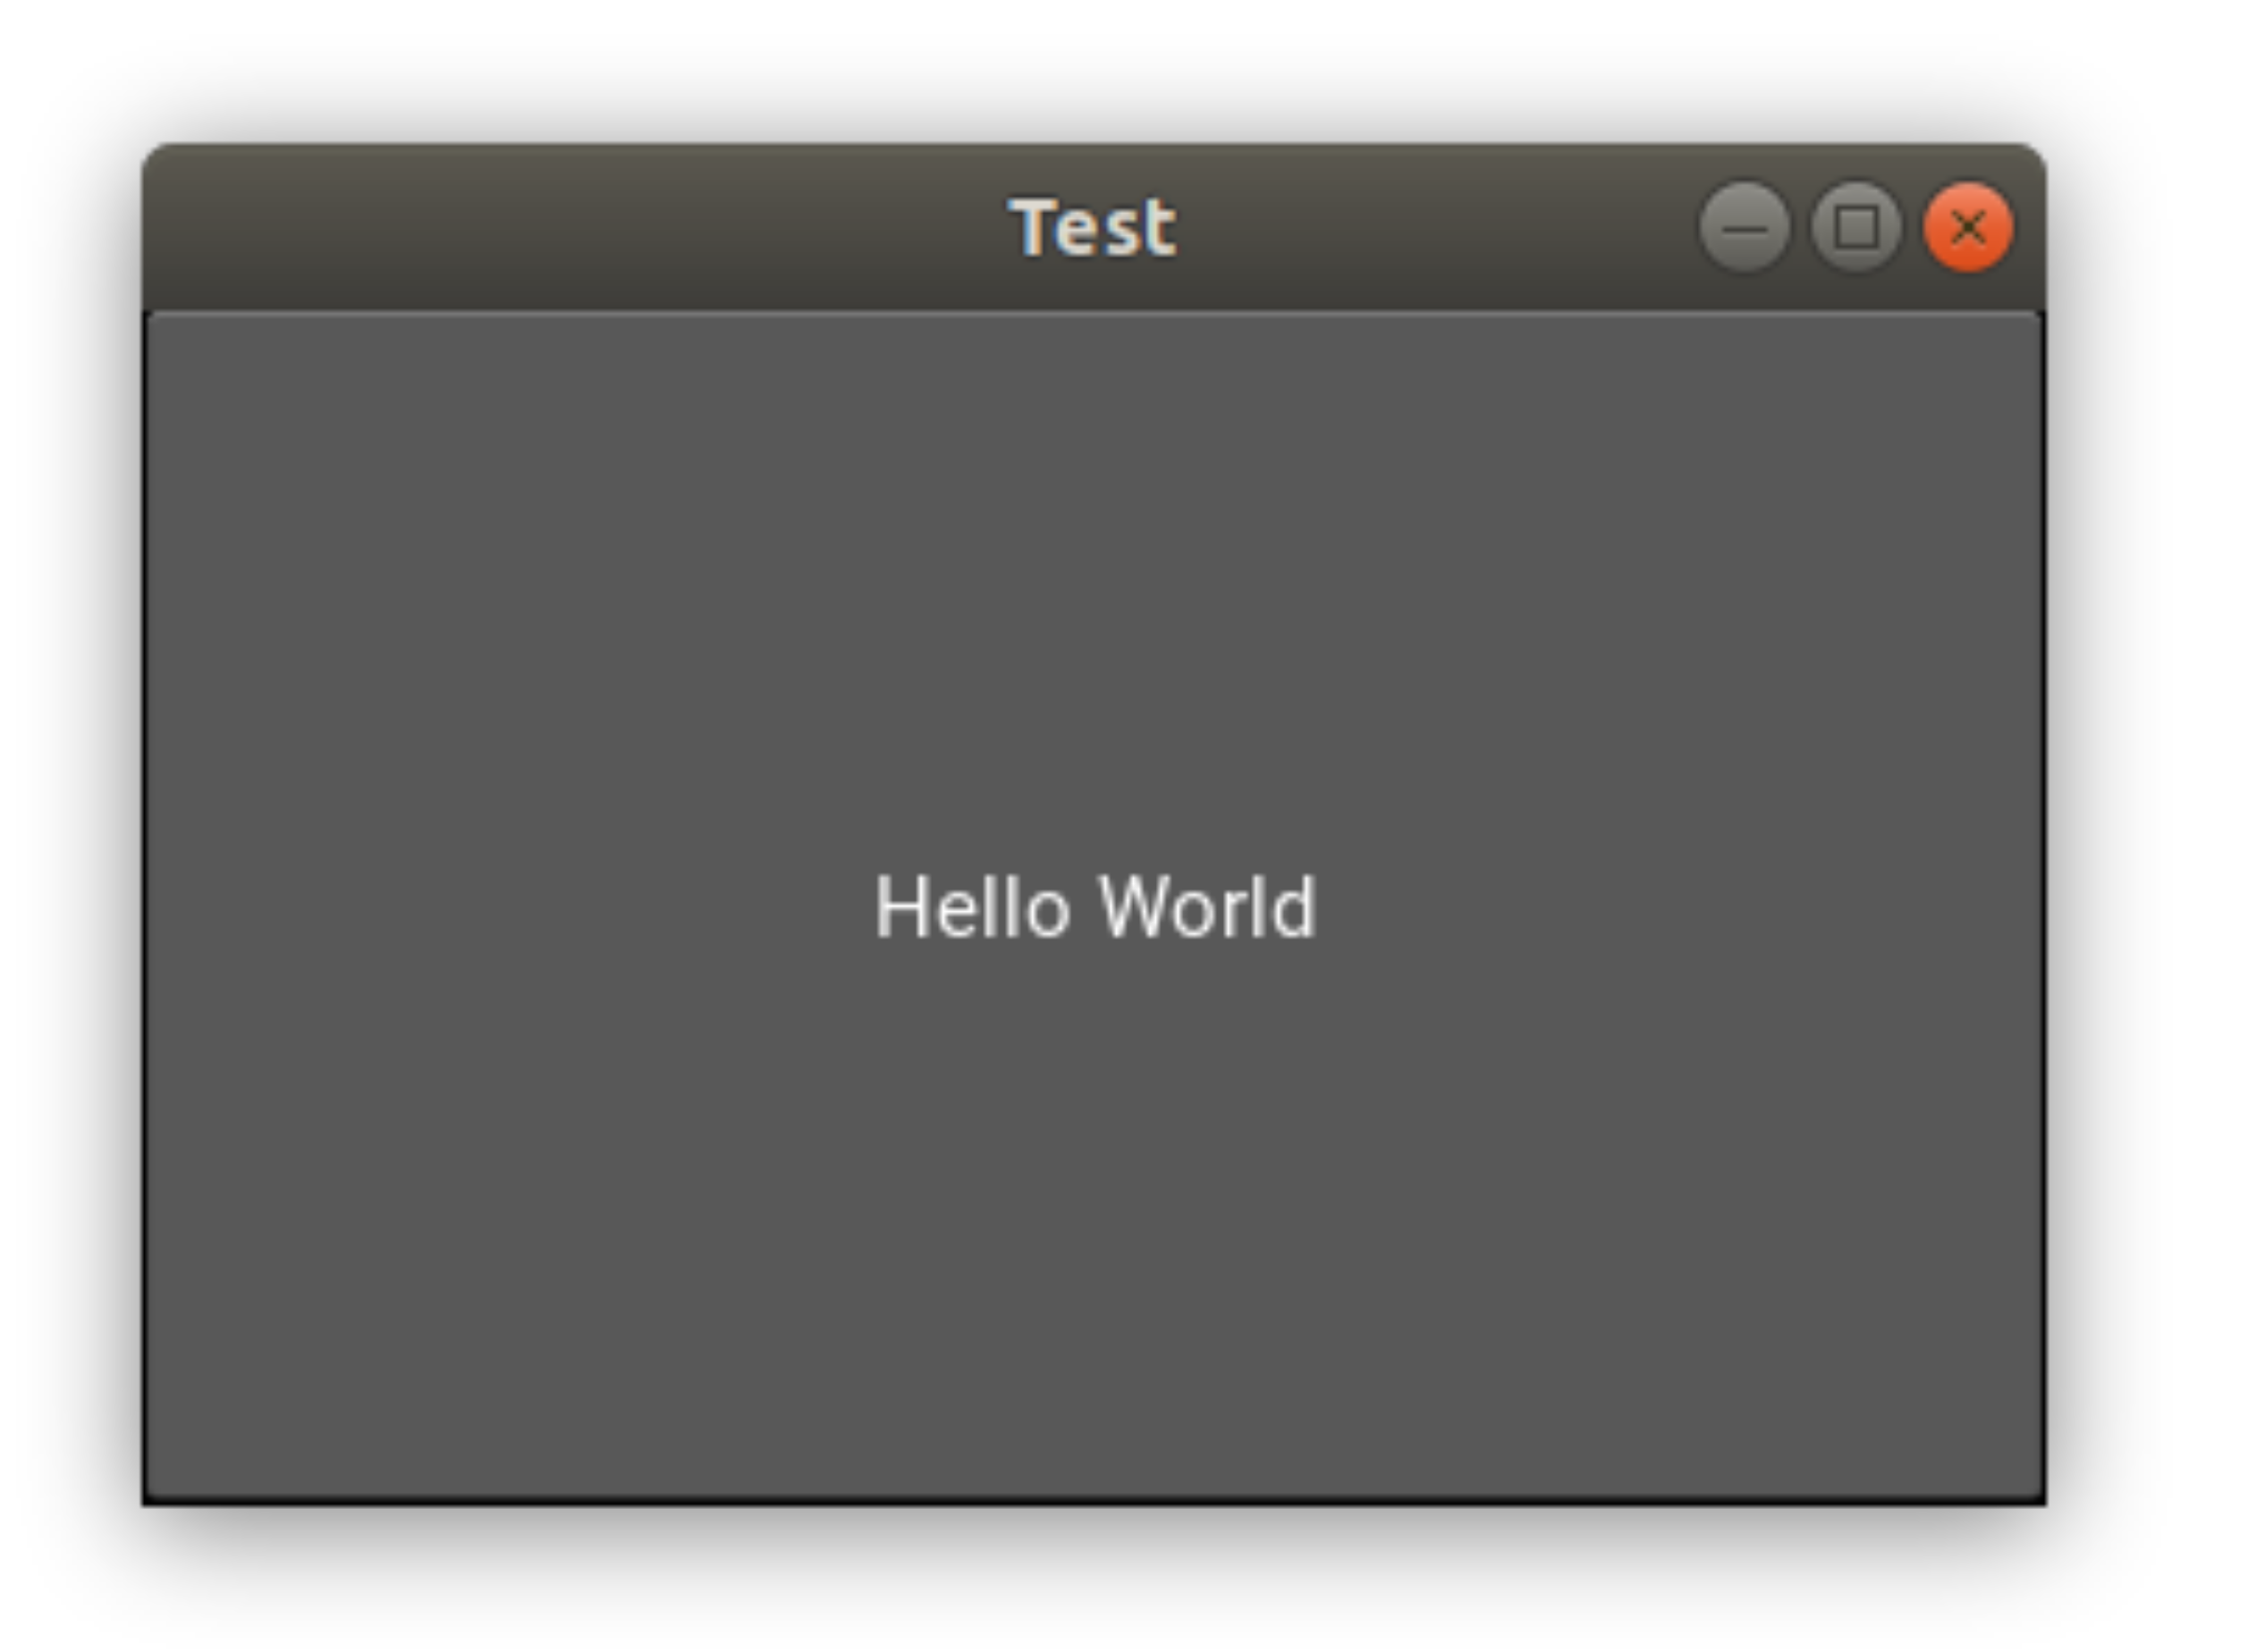
\includegraphics[width=7cm]{texto/fig/hello_world_kivy.png} 
                \end{center}
                \fonte{O Autor, 2018}
                \label{janela_kivy} 
            \end{figure}


            
            \subsubsection{Scipy, MatplotLib, Numpy}
            \label{lim_scipy}
            
            Scipy é um ecossistema de ferramentas para processamento de dados científicos contando com ferramentes de manipulação de matrizes, plotagem de gráficos, interpolação dentro outras ferramentas.
            
            Desenvolvido pela \citar{achar a organização} o ecossistema é de código aberto as principais ferramentas são: Numpy \citar{numpy} para trabalhos com vetores e matrizes, Matplotlib \citar{matplotlib} são ferramentas para plotagem de dados e o próprio Scipy para interpolação, cálculo de espectro de frequência dentre outras.
            
            A tabela \ref{pontos_ex_inter} apresenta 9 pontos distribuídos numa matriz quadrada de ordem 3, onde, a posição (2,2) possui uma anomalia, o código \citar{\ref{lim_scipy}.1} mostra como fazer a interpolação dos pontos e como plotar o resultado (figura \ref{fig_ex_inter}).
            
            
            \begin{table}[H]
                
                \caption{Distribuição de pontos com valor anômalo ao centro.}
                \label{pontos_ex_inter}
                \begin{center}
                    \centering
                    \begin{tabular}{l|ccc}
                        \hline
                        {\bf Ponto} & {\bf x} & {\bf y} & {\bf z}\\
                        \hline
                        1&1       &   1     &  1     \\
                        %\hline
                        2&2       &   1     &  1     \\
                        %\hline
                        3&3       &   1     &  1     \\
                        %\hline
                        4&1       &   2     &  1     \\
                        %\hline
                        5&2       &   2     &  3     \\
                        %\hline
                        6&3       &   2     &  1     \\
                        %\hline
                        7&1       &   3     &  1     \\
                        %\hline
                        8&2       &   3     &  1     \\
                        %\hline
                        9&3       &   3     &  1     \\
                        \hline
                    \end{tabular}
                \end{center}
                \fonte{O Autor, 2018}
            \end{table}
            
            Exemplo Numpy:
            \begin{quote}
             \codbox{\ini \cl{import} Numpy \cl{as} np        \\
                     \ini                                     \\
                     \ini  x = np.array([1,2,3,1,2,3,1,2,3])  \\
                     \ini  y = np.array([1,1,1,2,2,2,3,3,3])  \\
                     \ini  z = np.array([1,1,1,1,3,1,1,1,1])                                                                  
             }                                            \citar{\codnum{\ref{lim_scipy}.1}}
            \end{quote}
            
            Exemplo Scipy:
            
            \begin{quote}
             \codbox{\ini \cl{from} scipy \cl{import} interpolate              \\
                     \ini \cl{from} scipy.interpolate \cl{import} griddata     \\
                     \ini                                                      \\
                     \ini  xi = np.arange(x.min(), x.max(), .01)               \\
                     \ini  yi = np.arange(y.min(), y.max(), .01)               \\
                     \ini  xi,yi = meshgrid(xi,yi)                             \\
                     \ini                                                      \\
                     \ini  \cc{ Interpolate}                                   \\
                     \ini  zi = griddata((x,y),z,(xi,yi),\ob{method}=\st{'cubic'})       
             }                                                                    \citar{\codnum{cont. \ref{lim_scipy}.1}}
            \end{quote}
            
            Exemplo Matplotlib:
            
            \begin{quote}
             \codbox{\ini \cl{import} matplotlib.pyplot \cl{as} plt            \\
                     \ini                                                      \\
                     \ini  plt.figure(1)                                       \\
                     \ini  plt.subplot(111)                                    \\
                     \ini                                                      \\
                     \ini  zn = np.arange(z.min(), z.max() + 0.01, .01)        \\
                     \ini                                                      \\
                     \ini  plt.plot(x, y, \st{'kx'})                           \\
                     \ini  plt.contourf(xi, yi, zi, zn)                        \\
                     \ini  plt.colorbar()                                      \\ 
                     \ini  plt.grid()                                          \\
                     \ini  plt.set\_cmap(\st{'jet'})                            \\
                     \ini  plt.show()                                           \\
             }                                                                   \citar{\codnum{cont. \ref{lim_scipy}.1}}
            \end{quote}
            
            \begin{figure}[H]
                \caption{Exemplo dos pontos interpolados usando Scipy e plotados usando Matplotlib}
                \begin{center}
                    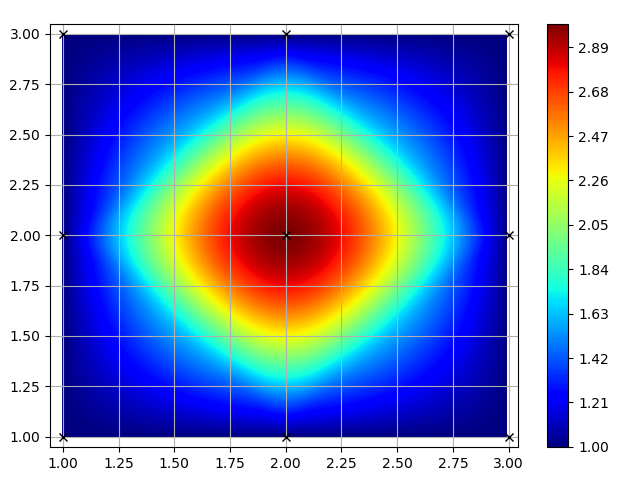
\includegraphics[width=10cm]{texto/fig/plot_ex.png} 
                \end{center}
                \fonte{O Autor, 2018}
                \label{fig_ex_inter} 
            \end{figure}
            
            
        \subsection{Pacotes de Processamentos do grupo Geoma - INPE}
    
    
    
    \section{Arquitetura do \textit{Software}}
    
        
    
